% !TeX spellcheck = nl_NL
\documentclass[a4paper,kulak]{kulakarticle} %options: kul or kulak (default)

\usepackage[dutch]{babel}
\usepackage{hyperref}
\usepackage{graphicx}
\usepackage{amsmath,amssymb,amsthm}
\usepackage{siunitx}
\usepackage{pdfpages}
\usepackage{subfig}

\date{Academiejaar 2020 -- 2021}
\address{
  Fysica doorstroomoptie ingenieurswetenschappen \\
  Probleemoplossen en ontwerpen, deel 1\\
  Stijn Rebry, Kevin Truyaert}
\title{Literatuurstudie}
\author{Mathis Bossuyt}


\begin{document}

\maketitle
\\
\section*{Welke rol speelt aerodynamica in Formule 1}
\section*{Inleiding}

In Formule 1 wordt er vaak gesproken over aerodynamica en downforce van de wagens, maar wat wordt daarmee bedoeld? In de eerste paragraaf zullen we deze termen verklaren en daarnaast ook enkele basisprincipes uit de aerodynamica gaan bekijken. in de tweede paragraaf gaan we dieper in op de sport en kijken we waar de uitdagingen voor de verschillende teams liggen. in de laatste paragraaf gaan we bekijken hoe downforce gecreëerd wordt bij de achtervleugel van een F1-wagen. 

\section{Enkele basisprincipes}

In dit gedeelte zullen we enkele termen verklaren en daarnaast enkele basisprincipes uit de aerodynamica en natuurkunde bekijken, zoals de wet Bernoulli en de derde wet van Newton.

\subsection{Aerodynamica en downforce}

\begin{itemize}
	
	\item Aerodynamica: Is een wetenschapstak die gaat kijken hoe gassen zich gedragen in de ruimte en meer bepaald in het bijzijn van een voorwerp.
	\cite{houghton2003aerodynamics}
	
	\item Downforce: De vertaling van downforce is neerwaartse kracht, deze kracht zal de wagen naar beneden duwen waardoor een wagen meer grip zal hebben op het wegdek. Wanneer een wagen grotere downforce ondervindt zal deze wagen als bijgevolg ook sneller een bocht kunnen nemen. 
	\cite{houghton2003aerodynamics}
	
\end{itemize}

\subsection{Wet van Bernoulli}

De wet van Bernoulli is 1 van de belangrijkste basisprincipes wanneer je spreekt over  de beweging van gassen en vloeistoffen. Wanneer een vloeistof of gas bijvoorbeeld door een leiding gaat en er plots een vernauwing is zal het gas of vloeistof een lagere druk ondervinden. Zoals je in de formule \ref{Bernoulli} , hieronder kan zien is de druk omgekeerd evenredig met de snelheid. daardoor zal het gas bij een vernauwing een lagere druk maar een hogere snelheid aannemen. In deze formule \ref{Bernoulli} is $\rho $ de massadichtheid, $g $ de valversnelling, $h $ de hoogte en $p $ de druk van het gas.
\\

\begin{equation}
\frac{ \rho v^2}{2}  + \rho gh + p = constante
\label{Bernoulli}
\end{equation}

\subsection{Derde wet van Newton}
De derde wet van Newton  \ref{Newton} speelt een belangrijke rol in de mechanica maar ook in de aerodynamica. een kracht op een deeltje gaat gepaard met een even grote maar tegengestelde kracht. 	\cite{houghton2003aerodynamics}

\begin{equation}
\vec{F}_{actie} = - \vec{F}_{reactie}
\label{Newton}	
\end{equation}

\section{Aerodynamica in Formule 1}
In de vorige paragraaf werden enkele begrippen en basisprincipes uitgelicht, die van belang zijn om de aerodynamica van een F1-wagen te begrijpen. Aerodynamica speelt een enorme rol, het reduceert de tijd om 1 ronde te rijden met 20 \% , dit is dan ook de uitleg waarom er zo veel wordt geïnvesteerd in het gestroomlijnder maken van de wagens. \cite{toet2013aerodynamics} \cite{zhang2004vortices}

\subsection{Downforce en drag} 
Het doel van de teams is om zo veel mogelijk downforce te creëren, zodat de wagen aan het wegdek blijft kleven. Het probleem met de downforce eindeloos te vergroten is dat je op een bepaald moment veel luchtweerstand krijgt, waardoor de auto vertraagt en dat is juist wat je wilde vermijden door een grotere downforce te creëren. De Ingenieurs en ontwerpers moeten dus op zoek naar een zo perfect mogelijke verhouding tussen luchtweerstand en de gecreëerde downforce.

\section{Downforce creatie door de achtervleugel van de wagen}

Een groot deel van de neerwaartse kracht wordt gecreëerd door de achtervleugel. Zoals je op de figuur \autoref{vleugel} kan zien heeft de vleugel een zeer specifiek vorm, dit is om de downforce te vergroten.
\\

Wanneer lucht tegen de deze vleugel aan botst zal de lucht zich gaan opsplitsen. Een deel zal langs de bovenkant van de vleugel voortbewegen en het ander deel zal langs de onderkant van de vleugel voortbewegen. De lucht die onder de vleugel voortbeweegt zal sneller bewegen omdat de lucht naar een vacuüm aan de achterkant van de vleugel, wordt getrokken die gecreëerd werd door de vleugel dit is te zien op \autoref{vleugel} .
\\

doordat de lucht sneller beweegt zal de druk er lager zijn, zie de wet van Bernoulli \ref{Bernoulli} . De vorm van de vleugel zorgt ervoor dat de lucht die zich boven de vleugel bevindt ook naar boven afbuigt, dit is ook zo voor het onderste deel van de lucht maar dit komt door het gecreëerde vacuüm.
\\

de luchtdeeltjes bewegen zich naar boven, maar zoals wij bij de basisprincipes zagen is er altijd een omgekeerde en evengrote reactiekracht \ref{Newton} , deze omgekeerde kracht die naar benenden wijst is de downforce. Deze kracht zorgt ervoor dat de wagen 'plakt' aan het wegdek. 
\\

De achtervleugel is maar een voorbeeld van de vele onderdelen die downforce creëren. Het is echter wel eenvoudig om te zien hoe deze gecreërd wordt, en werd daarom in dit artikel gekozen.
 







\begin{figure}[ht]
	\centering
	\begin{minipage}[b]{0.4\textwidth}
	\includegraphics[width=\textwidth]{rearwing}
			
	\end{minipage}
	\hfill
	\begin{minipage}[b]{0.4\textwidth}
	\includegraphics[width=\textwidth]{achtervleugel}
			
	\end{minipage}
	\caption{A downforce creatie achtervleugel \cite{zhang2006ground} \cite{taylor_2018}}
	\label{vleugel}
\end{figure}










\section*{Besluit}

We merken dat aerodynamica een enorme rol speelt in de Formule 1 wereld. Jaarlijks gaan er enorme bedragen naar het ontwikkelen van nieuwe onderdelen die de bolide nog gestroomlijnder maken. het gestroomlijnder maken van de wagen levert duidelijk op, de tijden verminderden door aerodynamica met 20 \% .





\bibliography{bibliografie_literatuurstudie}
\bibliographystyle{unsrt}


\clearpage
\section*{Analyse van 'Aerodynamics and aerodynamic research in Formula 1'}

\subsection{Plannen}
(b) Welke voorkennis verwacht de auteur van zijn doelpubliek?
\\

De auteur verwacht wel enige voorkennis. Hij verwacht dat je enige kennis van kinetica en aerodynamica hebt, daarnaast verwacht hij ook dat je enige achtergrondkennis hebt over Formule 1.
Dit merk je aan de begrippen die de auteur gebruikt, een leek zonder kennis heeft het moeilijker om deze tekst te begrijpen. 
\subsection{Ontwerpen}
(a) Kan de lezer op basis van de titel de inhoud van het artikel correct inschatten?
\\

Jazeker, de titel is zeer duidelijk en kan je niet mis opvatten. Je weet dat het over formule 1 zal gaan en meer bepaald het aerodynamisch aspect ervan.
\subsection{schrijven}
(c) Bekijk een willekeurige figuur uit het artikel en bepaal of deze los van de tekst correct geïnterpreteerd kan worden.
\\

Ik heb gekozen om figuur 7 te bekijken van het desbetreffende artikel. De figuur is in drie delen opgedeeld: een tabel over drag per onderdeel, een andere tabel over down force per onderdeel en illustratie van een F1-wagen waarbij de onderdelen ingekleurd zijn. Ik denk dat deze figuur zonder tekst correct kan geïnterpreteerd kan worden, je kan zien dat bepaalde onderdelen downforce creëren en andere drag veroorzaken en kan deze ook terugvinden op de wagen zelf aan de hand van de kleuren.
\subsection{Opmaken}
(d) Is kleurgebruik in het artikel functioneel (indien aanwezig) of wenselijk (indien afwezig)?
\\

Het grootste deel van de tekst bestaat uit grijswaarden en dit zorgt niet voor een verminderde leesbaarheid, zelfs niet bij de schijfdiagrammen. Er is gekozen om 1 tabel in kleur te zetten, wat ik eigenlijk onnodig vind. De tabel zou perfect leesbaar zijn als die in grijswaarden was gemaakt.
\subsection{Reviseren}
(a) Vanuit welke onderzoeksvragen kan het artikel zijn vertrokken? Ga na waar deze zijn beantwoord.
\begin{itemize}
	\item Welke onderdelen zorgen voor drag en welke voor downforce: p.12-13
	\item Ofdat aerodynamica een groot verschil maakt voor de sport: p.12
	\item waarom de sport blijft voort ontwikkelen: p.25
	\item welke krachten de agens afremmen: p.15-20
\end{itemize}

\clearpage

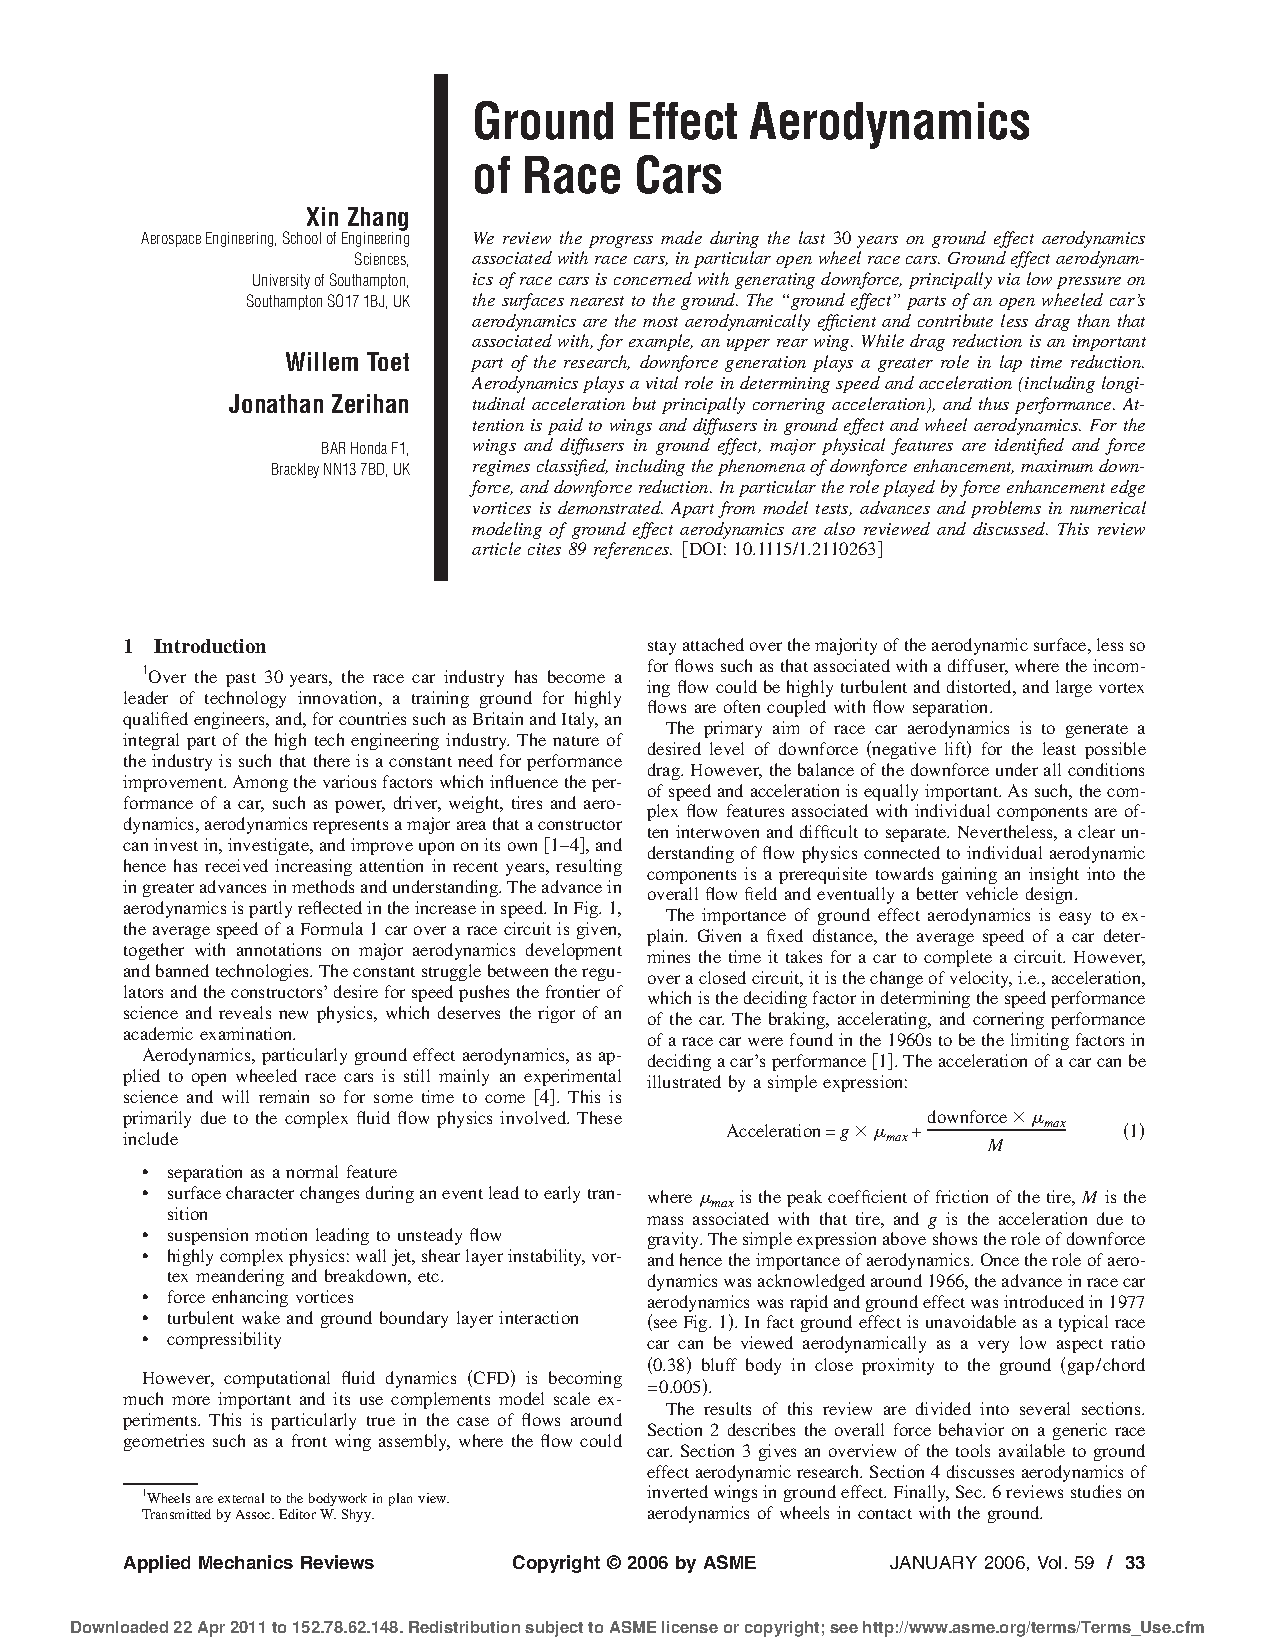
\includepdf[pages=1]{janm}
\clearpage

\includepdf[pages=1]{janp}
\clearpage

\includepdf[pages=1]{jann}
\end{document}
